\chapter{System Analysis}

\section{System Analysis}

\subsection{Requirement Analysis}

\subsubsection{Functional Requirements}

\begin{enumerate}
    \item The system shall accept a syllabus, chapter, or topic selection from the client application.
    \item The system shall retrieve the corresponding academic content from the vector database using semantic similarity search.
    \item The system shall construct a predefined prompt by combining the retrieved context with instructional guidelines.
    \item The system shall generate topic-specific explanations using a Large Language Model.
    \item The system shall return generated responses through a REST API in JSON format.
    \item The system shall support multiple subjects by maintaining separate academic knowledge bases.
    \item The system shall provide relevant and syllabus-oriented explanations based on the selected topic.
    \item The system shall allow preprocessing of academic PDF documents for vector database creation.
\end{enumerate}

\begin{figure}[ht]
    \centering
    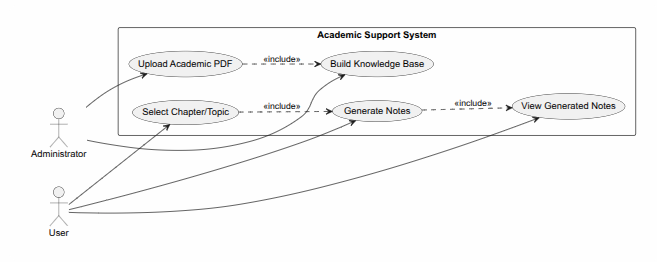
\includegraphics[width=0.6\textwidth]{figures/use-case-diagram.png}
    \caption{Use Case Diagram}
    \label{fig:use_case_diagram}
\end{figure}

\begin{table}[ht]
    \centering
    \caption{Build Knowledge Base Use Case}
    \label{tab:build_knowledge_base_use_case}

    \begin{tabular}{|c|l|}
        \hline
        Field & Description \\
        \hline
        Use Case ID & UC-1 \\
        Use Case Name & Build Knowledge Base \\
        Primary Actor & Administrator \\
        Description & Creates or updates the vector database from academic PDF documents.\\
        Preconditions & Academic PDF documents are available for processing. \\
        Postconditions & The vector database is updated with new embeddings. \\
        Main Flow & 
        \begin{minipage}[t]{10cm}
            \begin{enumerate}
                \item The administrator uploads academic documents.
                \item The system extracts textual content.
                \item The text is divided into chunks.
                \item Embeddings are generated.
                \item Embeddings are stored in the vector database.
            \end{enumerate}
        \end{minipage} \\
        Alternative Flow & If document processing fails, the system reports the error and terminates the indexing process. \\
        \hline
    \end{tabular}
\end{table}

% Table 2
\begin{table}[ht]
    \centering
    \caption{Generate Academic Response Use Case}
    \label{tab:generate_academic_response_use_case}

    \begin{tabular}{|c|l|}
        \hline
        Field & Description \\
        \hline
        Use Case ID & UC-2 \\
        Use Case Name & Generate Academic Response \\
        Primary Actor & Client Application \\
        Description & Generates a syllabus-oriented explanation for the selected chapter or topic.\\
        Preconditions & The academic knowledge base has been created and the client application provides the required request parameters. \\
        Postconditions & The generated response is returned to the client in JSON format. \\
        Main Flow &
        \begin{minipage}[t]{10cm}
            \begin{enumerate}
                \item The client application sends a request containing the syllabus, chapter, or topic information.
                \item The API validates the request.
                \item Relevant content is retrieved from the vector database.
                \item The retrieved context is combined with the predefined prompt.
                \item The LLM generates the response.
                \item The API returns the generated response.
            \end{enumerate} 
        \end{minipage} \\
        Alternative Flow & If no relevant content is found, the system returns an appropriate message indicating that no matching academic content is available. \\
        \hline
    \end{tabular}
\end{table}

\subsubsection{Non-Fucntional Requirements}

The non-functional requirements describe the quality attributes and operational characteristics expected from the proposed Academic Support System. \par

\paragraph{Performance}
The system shall generate and return academic responses within an acceptable response time under normal operating conditions. Semantic retrieval and response generation should be optimized to minimize user waiting time.

\paragraph{Reliability}
The system shall consistently generate accurate and contextually relevant responses based on the retrieved academic content. It should continue to function reliably as long as the required services and knowledge base are available.

\paragraph{Scalability}
The system shall support the addition of new academic subjects, chapters, and documents without requiring significant modifications to the existing architecture.

\paragraph{Maintainability}
The system shall be modular so that components such as document preprocessing, embedding generation, vector storage, and response generation can be updated or maintained independently.

\paragraph{Usability}
The system shall provide a simple REST API that can be easily integrated with external frontend or backend applications. The API should accept structured requests and return responses in a standardized JSON format.

\paragraph{Availability}
The system shall remain available for processing requests whenever the backend server, vector database, and Large Language Model service are operational.

\paragraph{Security}
The system shall validate incoming API requests and handle invalid or incomplete inputs appropriately to ensure reliable operation and prevent unexpected failures.


\subsection{Feasibility Analysis}
\subsubsection{Technical Feasibility}
The proposed Academic Support System is technically feasible as it is developed using Python, FastAPI, PyPDFLoader, Sentence Transformers, Qdrant, and the Gemini API. These technologies provide the required capabilities for document processing, semantic embedding generation, vector storage, information retrieval, and AI-based response generation. The system is developed on standard computing hardware without requiring specialized infrastructure, making it suitable for academic and institutional use. \par

\subsubsection{Operational Feasibility}
The system is operationally feasible as it provides REST API endpoints that can be  integrated with external applications to deliver syllabus-oriented academic assistance.  Administrators can build and update the knowledge base by processing academic documents, while client applications can request AI-generated explanations based on the  selected syllabus, chapter, or topic. The modular design simplifies maintenance and future  integration. \par

\subsubsection{Economic Feasibility}
The development cost of the proposed system is relatively low because it utilizes open-source technologies and freely available development tools. Python, FastAPI, Qdrant, and other supporting libraries do not require licensing costs. The system uses the free-tier Gemini API for response generation, resulting in minimal operational cost. Therefore, the overall project is economically feasible. \par

\subsubsection{Schedule Feasibility}
The project is schedule feasible as it can be completed within the allocated academic timeframe. The development process was organized into requirement analysis, literature review, system design, implementation, testing, and documentation phases. Proper planning and resource management ensured the timely completion of each project milestone. \par

\subsection{Object-Oriented Analysis}

\subsubsection{Object Modelling using Class and Object Diagrams}
The class diagram illustrates the structural organization of the proposed Academic Support System and the relationships among its major software components. The system follows a modular architecture consisting of service classes and adapter classes. The IngestionService is responsible for processing academic documents, generating embeddings, and storing vector representations in the vector database. The RetrievalService performs semantic retrieval by generating embeddings for the requested topic and searching the vector database for relevant content. The GenerationService constructs prompts using the retrieved context and invokes the language model to generate academic explanations. \par

To improve modularity and extensibility, the system employs abstraction through the EmbeddingAdapter, VectorDBAdapter, and LLMAdapter abstract classes. Their concrete implementations\texttt{--} SentenceTransformersAdapter, QdrantAdapter, and GeminiAdapter\texttt{--} provide the actual embedding generation, vector database operations, and language model interactions, respectively. This design reduces coupling between components, promotes code reusability, and allows different implementations to be substituted with minimal changes to the core services. \par

The Object Diagram represents a runtime snapshot of the Academic Support System, illustrating the instantiated objects and their relationships during system execution. Unlike the Class Diagram, which presents the static structure of the system, the Object Diagram depicts actual instances of the service and adapter classes. The service (for ingestion service), \texttt{retrieval\_service}, and \texttt{generation\_service} objects collaborate with the SentenceTransformersAdapter, VectorDBAdapter, and LLMAdapter objects to perform document ingestion, semantic retrieval, vector database operations, and AI-based response generation. This diagram demonstrates how the instantiated components interact to support the execution of the Retrieval-Augmented Generation (RAG) pipeline. \par

\begin{figure}[ht]
    \centering
    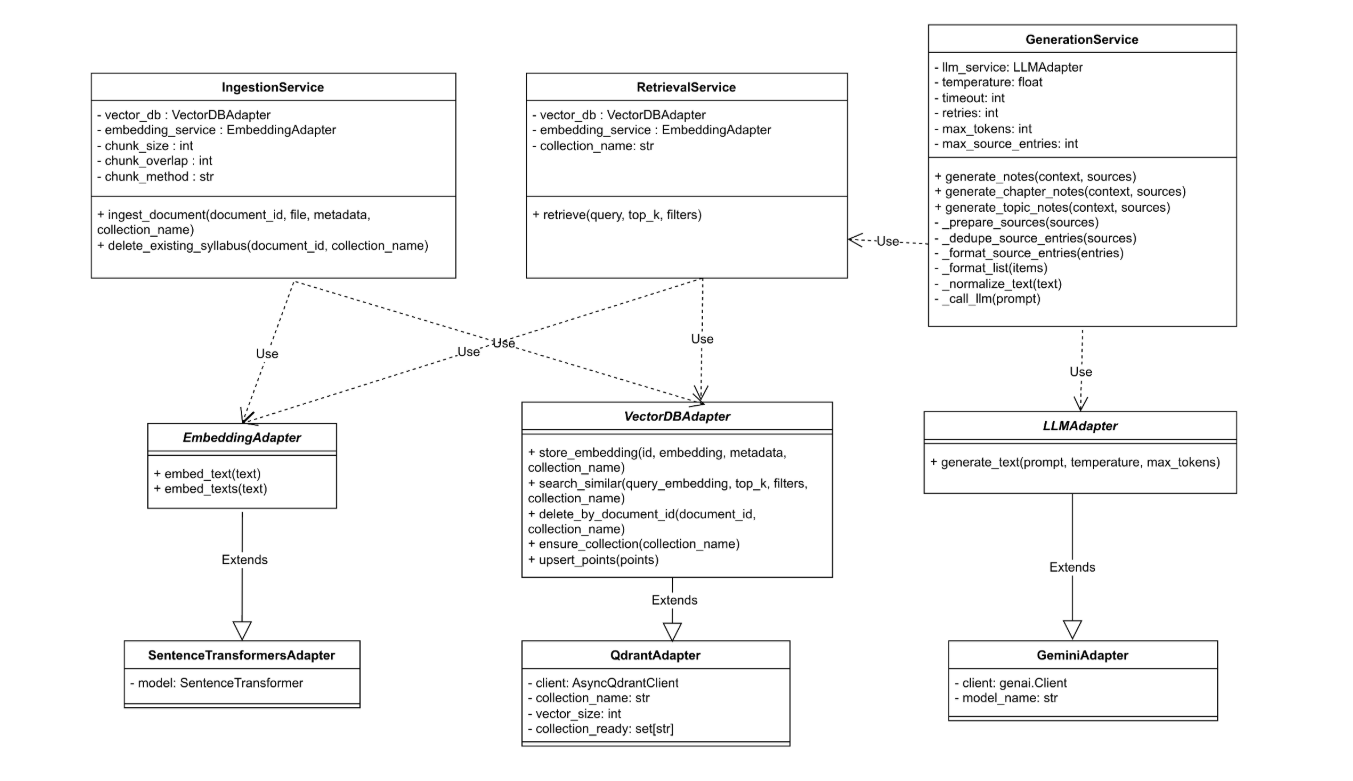
\includegraphics[width=0.8\textwidth]{figures/class-diagram.png}
    \caption{Class Diagram}
    \label{fig:classdiagram}
\end{figure}